%%
% Modificación de una plantilla de Latex para adaptarla al castellano.
%%

%%%%%%%%%%%%%%%%%%%%%
% Thin Sectioned Essay
% LaTeX Template
% Version 1.0 (3/8/13)
%
% This template has been downloaded from:
% http://www.LaTeXTemplates.com
%
% Original Author:
% Nicolas Diaz (nsdiaz@uc.cl) with extensive modifications by:
% Vel (vel@latextemplates.com)
%
% License:
% CC BY-NC-SA 3.0 (http://creativecommons.org/licenses/by-nc-sa/3.0/)
%
%%%%%%%%%%%%%%%%%%%%%

%----------------------------------------------------------------------------------------
%	PACKAGES AND OTHER DOCUMENT CONFIGURATIONS
%----------------------------------------------------------------------------------------

\documentclass[a4paper, 10pt]{article} % Font size (can be 10pt, 11pt or 12pt) and paper size (remove a4paper for US letter paper)
\usepackage{helvet}
\renewcommand{\familydefault}{\sfdefault}
\usepackage[protrusion=true,expansion=true]{microtype} % Better typography
\usepackage{graphicx} % Required for including pictures
\usepackage[usenames,dvipsnames]{color} % Coloring code
\usepackage{wrapfig} % Allows in-line images
\usepackage[utf8]{inputenc}
\usepackage{enumerate}
\usepackage{enumitem}

% Imágenes
\usepackage{graphicx} 

\usepackage{amsmath}
% para importar svg
%\usepackage[generate=all]{svgfig}

% sudo apt-get install texlive-lang-spanish
\usepackage[spanish]{babel} % English language/hyphenation
\selectlanguage{spanish}
% Hay que pelearse con babel-spanish para el alineamiento del punto decimal
\decimalpoint
\usepackage{dcolumn}
\newcolumntype{d}[1]{D{.}{\esperiod}{#1}}
\makeatletter
\addto\shorthandsspanish{\let\esperiod\es@period@code}
\makeatother

\usepackage{longtable}
\usepackage{tabu}
\usepackage{supertabular}

\usepackage{multicol}
\newsavebox\ltmcbox

% Para algoritmos
\usepackage{algorithm}
\usepackage{algorithmic}
\usepackage{amsthm}

% Para matrices
\usepackage{amsmath}

% Símbolos matemáticos
\usepackage{amssymb}
\usepackage{accents}
\let\oldemptyset\emptyset
\let\emptyset\varnothing

\usepackage[hidelinks]{hyperref}

\usepackage[section]{placeins} % Para gráficas en su sección.
\usepackage[T1]{fontenc} % Required for accented characters
\newenvironment{allintypewriter}{\ttfamily}{\par}
\setlength{\parindent}{0pt}
\parskip=8pt
\linespread{1.05} % Change line spacing here, Palatino benefits from a slight increase by default

\makeatletter
\renewcommand\@biblabel[1]{\textbf{#1.}} % Change the square brackets for each bibliography item from '[1]' to '1.'
\renewcommand{\@listI}{\itemsep=0pt} % Reduce the space between items in the itemize and enumerate environments and the bibliography
\newcommand{\imagen}[2]{\begin{center} \includegraphics[width=90mm]{#1} \\#2 \end{center}}
\newcommand{\RFC}[1]{\href{https://www.ietf.org/rfc/rfc#1.txt}{RFC-#1}}

\renewcommand{\maketitle}{ % Customize the title - do not edit title and author name here, see the TITLE block below
\begin{center} % Center align
{\Huge\@title} % Increase the font size of the title
\end{center}

\vspace{20pt} % Some vertical space between the title and author name

\begin{flushright} % Right align
{\large\@author} % Author name
\\\@date % Date

\vspace{40pt} % Some vertical space between the author block and abstract
\end{flushright}
\renewcommand{\baselinestretch}{0.5}

}
%----------------------------------------------------------------------------------------
%	TITLE
%----------------------------------------------------------------------------------------

\title{\textbf{Ingeniería de Servidores\\Práctica 5: Ajuste del Sistema}\\ % Title
\vspace{20 pt}
Cuestiones de la Práctica 5} % Subtitle

\author{\textsc{Adrián Portillo Sánchez} % Author
\\{\textit{Universidad de Granada}}} % Institution

\date{\today} % Date

%----------------------------------------------------------------------------------------
\setcounter{secnumdepth}{0}
\usepackage{anysize}
\marginsize{3cm}{3cm}{2.5cm}{2.5cm}

\begin{document}
\thispagestyle{empty}
\maketitle
\pagebreak
\thispagestyle{empty}
\tableofcontents
\pagebreak
\listoffigures
\pagebreak

\section{Cuestión 1}
\textbf{Al modificar los valores del kernel de este modo, no logramos que persistan después de reiniciar la máquina. ¿Qué archivo hay que editar para que los cambios sean permanentes?.}\\

Para que los cambios sean permanentes el archivo que debemos editar es \textit{'/etc/sysctl.conf'}. \cite{1}
También el comando sysctl nos permite modificar parámetros en tiempo de ejecución, podemos usar \textit{'sysctl -a} para ver la lista de parámetros actuales.

\begin{figure}[H]
\centering 
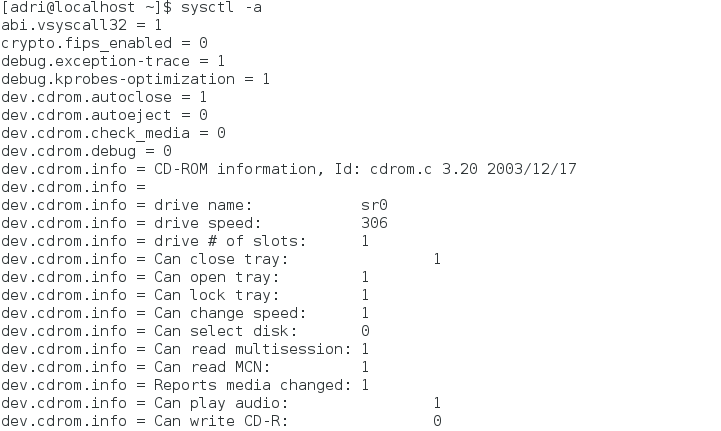
\includegraphics[width=1\linewidth]{sysctl1.png} 
\caption{Ejecución del comando sysctl -a en CentOS.} 
\label{contexto:figura} 
\end{figure}

Para modificar el archivo \textit{'/etc/sysctl.conf'} podemos utilizar cualquier editor de texto que nos proporciona el sistema, o también podemos modificarlo usando el comando sysctl ; por ejemplo, el resultado de ejecutar
\begin{verbatim}
    # sysctl -w kernel.hostname=pcadri
\end{verbatim}
será cambiar el nombre del equipo, que se hará válido una vez se reinicie el sistema.

\begin{figure}[H]
\centering 
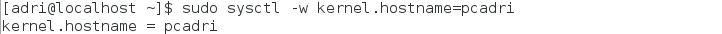
\includegraphics[width=1\linewidth]{sysctl2.png} 
\caption{Ejecución de la orden de sysctl en CentOS.} 
\label{contexto:figura} 
\end{figure}

\pagebreak

\section{Cuestión 2.}
\textbf{¿Con qué opción se muestran todos los parámetros modificables en tiempo de ejecución? Elija dos parámetros y explique, en dos líneas, qué función tienen.}\\

Para mostrar todos los parámetros modificables en tiempo de ejecución deberemos introducir \textit{sysctl –a}. Entre los obtenidos, podemos encontrar\cite{2}:

\begin{itemize}
    \item \textbf{kernel.pid\_max:} nos permite modificar el máximo valor valido para un PID de proceso en ejecución.
    \item \textbf{kernel.threads-max:} nos permite modificar el número de procesos máximos que se pueden ejecutar concurrentemente en el kernel.
\end{itemize}

\section{Cuestión 3.}
\textbf{Realice una copia de seguridad del registro y restáurela, ilustre el proceso con capturas.}\\

Para editar el registro en Windows podremos utilizar el editor del registro \textbf{'regedit'} \cite{3}, para crear la copia de seguridad podremos exportar el registro, y para restaurarlo importamos ese mismo registro exportado.

\begin{figure}[H]
\centering 
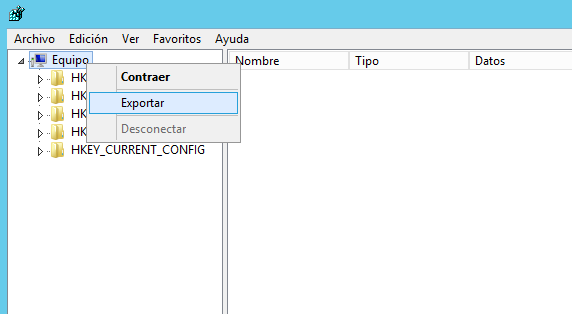
\includegraphics[width=1\linewidth]{reg1.png} 
\caption{Editor del registro en Windows.} 
\label{contexto:figura} 
\end{figure}

\begin{figure}[H]
\centering 
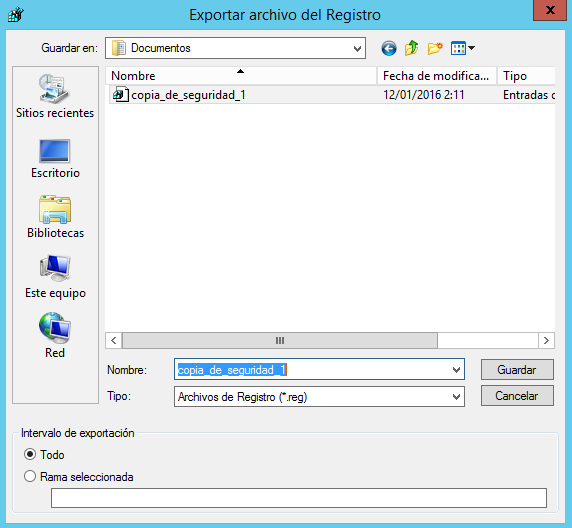
\includegraphics[width=0.85\linewidth]{reg2.png} 
\caption{Haciendo una copia de seguridad del registro. (Archivo -> Exportar)} 
\label{contexto:figura} 
\end{figure}


\begin{figure}[H]
\centering 
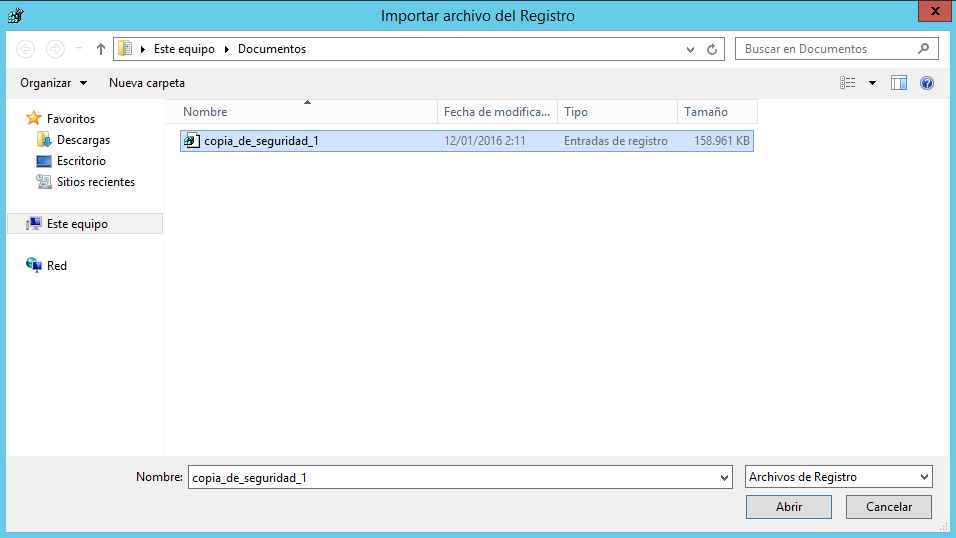
\includegraphics[width=0.85\linewidth]{reg3.png} 
\caption{Restaurando la copia de seguridad del registro. (Archivo -> Importar)} 
\label{contexto:figura} 
\end{figure}

\pagebreak

\section{Cuestión 4.}
\textbf{¿Cómo se abre una consola en Windows? ¿Qué comando hay que ejecutar para editar el registro? Muestre su ejecución con capturas de pantalla.}\\

Para abrir la consola en Windows deberemos acceder a la ventana \textbf{'Ejecutar'}, dicha ventana podemos abrirla desde \textbf{Menú Inicio -> Ejecutar} o utilizando la combinación de teclas \textbf{'Tecla Windows + R'}. Una vez en Ejecutar, debemos introducir \textit{cmd} y se abrirá la consola.

\begin{figure}[H]
\centering 
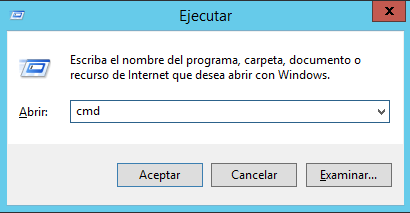
\includegraphics[width=0.85\linewidth]{cmd1.png} 
\caption{Abriendo la consola en Windows.} 
\label{contexto:figura} 
\end{figure}

Ahora para editar el registro debemos ejecutar el comando \textit{reg} \cite{4}.

\begin{figure}[H]
\centering 
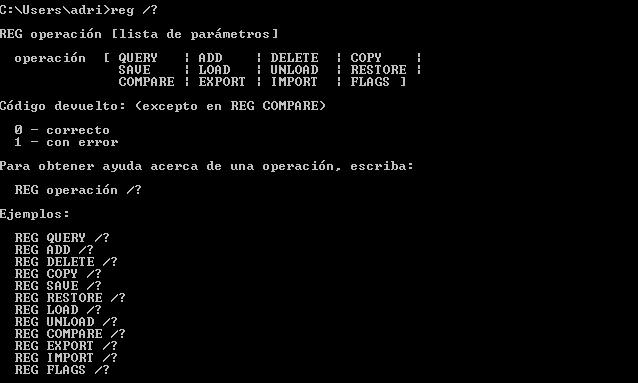
\includegraphics[width=0.85\linewidth]{cmd2.png} 
\caption{Distintas opciones para reg.} 
\label{contexto:figura} 
\end{figure}

\pagebreak

\section{Cuestión 5.}
\textbf{Las cadenas de caracteres y valores numéricos tienen distintos tipos. Busque en la documentación de Microsoft y liste todos los tipos de valores.}\\

\begin{itemize}
    \item \textbf{Valor binario [REG\_BINARY]:} datos binarios sin formato.
    \item \textbf{Valor DWORD [REG\_DWORD]:} datos representados por un número de 4 bytes de longitud (un valor entero de 32 bits).
    \item \textbf{Valor alfanumérico expandible [REG\_EXPAND\_SZ]:} Cadena de datos de longitud variable.
    \item \textbf{Valor de cadena múltiple [REG\_MULTI\_SZ]:} Cadena múltiple.
    \item \textbf{Valor de cadena [REG\_SZ]:} Cadena de texto de longitud fija.
    \item \textbf{Valor binario [REG\_RESOURCE\_REQUIREMENTS\_LIST]:} Serie de matrices anidadas diseñara para almacenar una lista de recursos utilizados por el controlador de un dispositivo de hardware o uno de los dispositivos físicos que controla.
    \item \textbf{Valor binario [REG\_RESOURCE\_REQUIREMENTS\_LIST]:} Serie de matrices anidadas diseñara para almacenar una lista de recursos utilizados por el controlador de un dispositivo de hardware o uno de los dispositivos físicos que controla.
    \item \textbf{Valor binario [REG\_FULL\_RESOURCE\_DESCRIPTOR]:} Serie de matrices anidadas diseñada para almacenar una lista de recursos utilizados por un dispositivo físico de hardware.
    \item \textbf{Ninguna [REG\_NONE]:} Datos sin ningún tipo en particular.
    \item \textbf{Vínculo [REG\_LINK]:} Cadena Unicode que da nombre a un vínculo simbólico.
    \item \textbf{Valor QWORD [REG\_QWORD]:} Datos representados por un número entero de 64 bytes.
\end{itemize}
Información extraída de la fuente oficial \cite{5}.

\pagebreak

\section{Cuestión 6.}
\textbf{Enumere qué elementos se pueden configurar en Apache y en IIS para que Moodle funcione mejor.}\\

Los elementos configurables que podemos tener en cuenta para que Moodle funcione mejor son los siguientes \cite{6}:

\begin{itemize}

    \item En un servidor \textbf{Apache}:
    
    \begin{itemize}
        \item Ajustar el parámetro \textbf{'MaxClients'} en función de la memoria total disponible en nuestro equipo.
        \item Cargar el mínimo número posible de módulos para reducir la memoria necesaria.
        \item Utilizar la última versión de Apache porque reduce el uso de memoria.
        \item Reducir a un mínimo valor de 20-30 el parámetro \textbf{'MaxRequestPerChild'}, para que la bifurcación de procesos no genere una mayor sobrecarga en vez de beneficio en el rendimiento.
        \item Establecer el parámetro \textbf{'KeepAlive'} a Off o bajar el valor de \textbf{'KeepAliveTimeout'} a un valor de 2-5, evitando así sobrecarga del procesador en el inicio de proesos.
        \item En lugar de la anterior, podemos crear un servidor proxy inverso delante del servidor de Moodle para almacenar en caché los archivos HTML con imágenes.
        \item Si no utilizamos un archivo \textbf{'.htaccess'} establecer \textbf{'AllowOverride'} a None para no tener que buscar dichos archivos.
        \item Establecer correctamente \textbf{'DirectoryIndex'} para evitar negociación de contenido indicando el archivo de índice que debe ser cargado.
        \item Configurar \textbf{'ExtendedStatus'} a Off y desactivar \textbf{'mod\_info'} y \textbf{'mod\_status'} si no vamos a hacer trabajo de desarrollo en el servidor.
        \item No cambiar \textbf{'HostnameLookups'} de Off para reducir la latencia de DNS.
        \item Reducir \textbf{'TimeOut'} a 30-60 segundos.
        \item En las directivas \textbf{'Options'}, evitar \textbf{'Options MultiViews'} para reducir el uso de entrada/salida en disco.
    \end{itemize}
    
    \item En un servidor \textbf{ISS}:
    
    \begin{itemize}
        \item Ajustar a 2-5 el valor de \textbf{'ListenBacklog'}.
        \item Cambiar el \textbf{'MemCacheSize'} para ajustar la memoria que se usará como caché de archivos.
        \item Cambiar \textbf{'MaxCachedFileSize'} para ajustar el tamaño máximo de un archivo en la caché de archivos.
        \item Crear un valor DWORD llamado \textbf{'ObjectCacheTTL'} para cambiar la cantidad de tiempo (en milisegundos) que los objetos de la caché se mantienen en la memoria.
    \end{itemize}
\end{itemize}

\pagebreak

\section{Cuestión 7.}
\textbf{Ajuste la compresión en el servidor y analice su comportamiento usando varios valores para el tamaño a de archivo partir
del cual comprimir. Para comprobar que está comprimiendo puede usar el navegador o comandos como curl (see url) o lynx. Muestre capturas de pantalla de todo el proceso.}\\

Para ajustar la compresión en el servidor primero deberemos habilitar la compresión en el servidor \cite{7}, nos movemos hasta el directorio \textit{\%windir\%$\backslash$system32$\backslash$inetsrv} y ejecutaremos \textit{appcmd}, para habilitar la compresión de contenido dinámico ejecutamos
\begin{verbatim}
    appcmd set config /section:urlCompression /doDynamicCompression:True
\end{verbatim}
 y para habilitar la compresión de contenido estático ejecutamos
\begin{verbatim}
    appcmd set config /section:urlCompression /doStaticCompression:True
\end{verbatim}

\begin{figure}[H]
\centering 
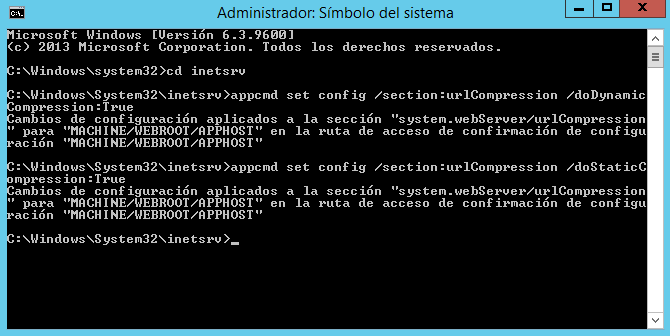
\includegraphics[width=1\linewidth]{inetsrv1.png} 
\caption{Ajustando la compresión del servidor.} 
\label{contexto:figura} 
\end{figure}

Para configurar la compresión accedemos al \textbf{'Administrador de Internet Information Services (ISS)'} desde \textbf{'Inicio -> Todos los programas -> Herramientas administrativas'}. Una vez ahí, seleccionamos el servidor (WIN-1RJ1IQJL3J0 es nuestro caso) y pulsamos \textbf{'Compresión'} para acceder a su ventana de configuración. Ahora marcamos la casilla \textbf{'Habilitar compresión de contenido estático'}, porque es la única que nos permite hacerlo, y rellenamos los campos inferiores.

\begin{figure}[H]
\centering 
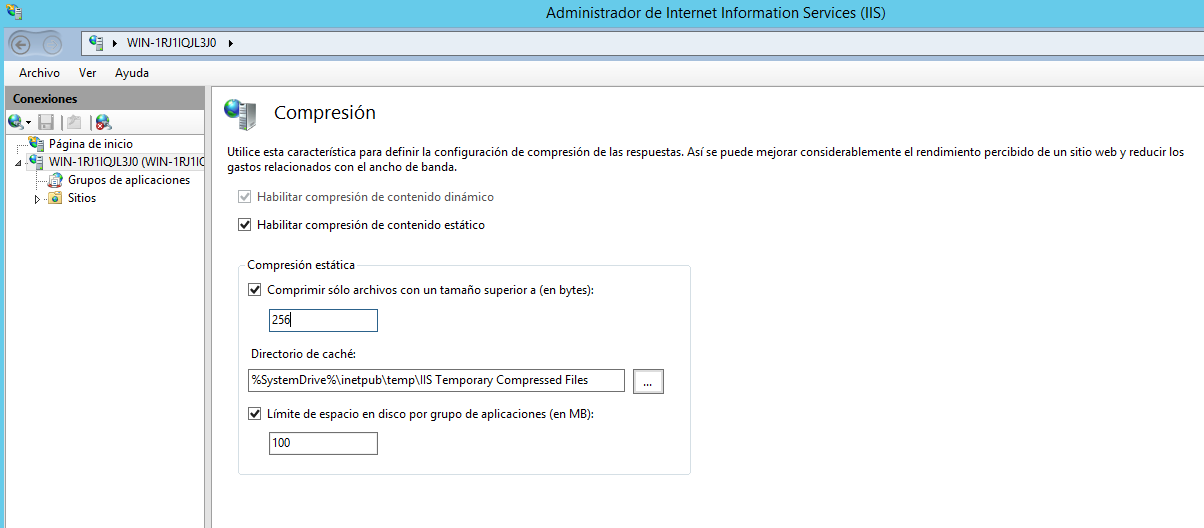
\includegraphics[width=1\linewidth]{inetsrv2.png} 
\caption{Configurando la compresión del servidor.} 
\label{contexto:figura} 
\end{figure}

Utilizando el complemento \textbf{Firebug} para \textbf{Firefox} \cite{8}, podemos ver el contenido de las cabeceras que se generan para la solicitud y la respuesta durante una comunicación entre un navegador y un servidor, como no he conseguido que funcione la compresión en el servidor IIS de mi propia máquina virtual, he hecho la prueba accediendo a la página de Facebook para poder ver cómo sería la respuesta de un servidor que acepta compresión. Vemos que la compresión es aceptada porque en el encabezado de respuesta aparece \textbf{Content-Encoding gzip} y en el encabezado de solicitud aparece \textbf{Accept-Encoding gzip, deflate}.

\begin{figure}[H]
\centering 
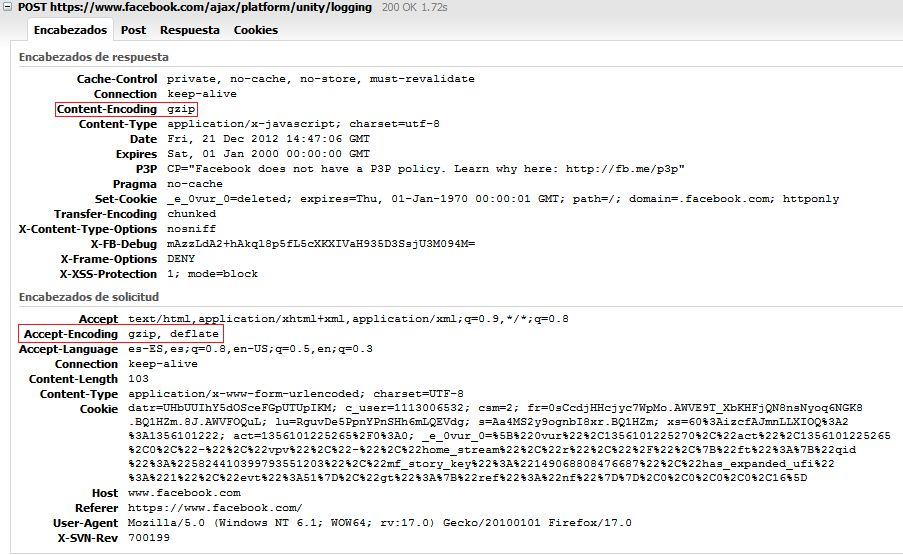
\includegraphics[width=1\linewidth]{inetsrv3.png} 
\caption{Observando los resultados de los cambios en un caso práctico.} 
\label{contexto:figura} 
\end{figure}

\pagebreak

\section{Cuestión 8.}
\textbf{Usted parte de un SO con ciertos parámetros definidos en la instalación (Práctica 1), ya sabe instalar servicios (Práctica 2) y cómo monitorizarlos (Práctica 3) cuando los somete a cargas (Práctica 4). Al igual que ha visto cómo se puede mejorar un servidor web (Práctica 5 Sección 3.1), elija un servicio (el que usted quiera) y modifique un parámetro para mejorar su comportamiento. (9.b) Monitorice el servicio antes y después de la modificación del parámetro aplicando cargas al sistema (antes y después) mostrando los resultados de la monitorización.}\\

He elegido modificar parámetros del servicio de Apache partiendo de las mejoras de Moodle de las Cuestión 6. Para hacerlo ejecutamos como root el archivo de configuración de Apache desde un editor de texto. En mi caso:

\begin{verbatim}
    sudo gedit /etc/apache2/apache2.conf
\end{verbatim}

Modifico los siguientes parámetros:

\begin{verbatim}
    KeepAlive On -> KeepAlive Off
    MaxKeepAliveRequests 100 -> MaxKeepAliveRequests 200
    KeepAliveTimeout 5 -> KeepAliveTimeout 2
\end{verbatim}
Los resultados antes de las modificaciones de:
\begin{verbatim}
    # ab -n 20000 -c 20 http://192.168.1.34/
\end{verbatim}

\begin{figure}[H]
\centering 
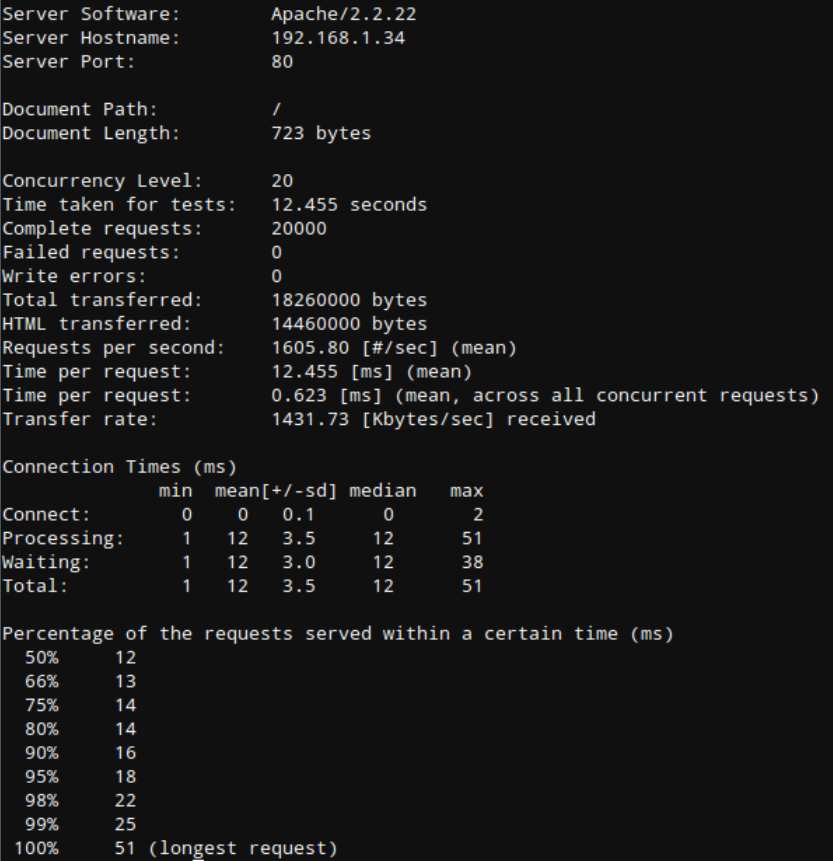
\includegraphics[width=0.65\linewidth]{apache1.png} 
\caption{Resultados de ab antes de las modificaciones.} 
\label{contexto:figura} 
\end{figure}

Después de las modificaciones:

\begin{figure}[H]
\centering 
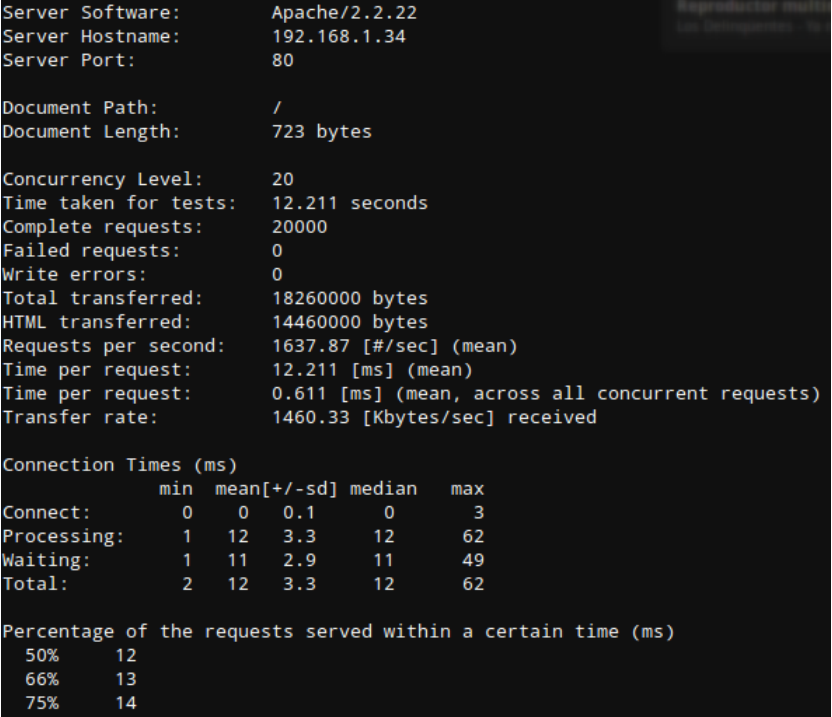
\includegraphics[width=1\linewidth]{apache2.png} 
\caption{Resultados de ab después de las modificaciones.} 
\label{contexto:figura} 
\end{figure} 

\pagebreak

\section{Cuestión Opcional 1.}
\textbf{Realice lo mismo que en la cuestión 8 pero para otro servicio.}\\

En este caso supondremos que tenemos un servidor algo escaso en memoria, por lo que querremos optimizar el uso de ram en todos los servicios posibles, en este caso intentaremos mejorar MySQL.

\begin{verbatim}
    mysql> use information_schema ;
    mysql> select * from ENGINES;
\end{verbatim}

\begin{figure}[H]
\centering 
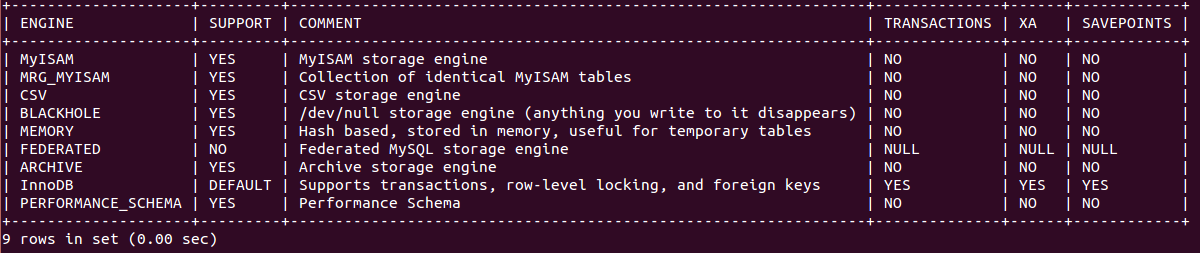
\includegraphics[width=1\linewidth]{sql1.png} 
\caption{Vista de los motores MySQL configurados.} 
\label{contexto:figura} 
\end{figure} 

Compararé el rendimiento utilizando un benchmark sencillo para los monitores de almacenamiento INNODB y MyISAM. Para ello usaré el comando mysqlslap \cite{9}:

\begin{verbatim}
    mysqlslap --user=root --auto-generate-sql -vv --concurrency=100
     --number-of-queries=10000 --engine=innodb -p
     
    mysqlslap --user=root --auto-generate-sql -vv --concurrency=100
     --number-of-queries=10000 --engine=myisam -p
\end{verbatim}

Este test hace algo similar al que vimos con el comando ab para Apache, realiza peticiones concurrentemente al servidor MySQL. Para este estudio realizaremos 10000 peticiones con una concurrencia de 100 conexiones.

\begin{figure}[H]
\centering 
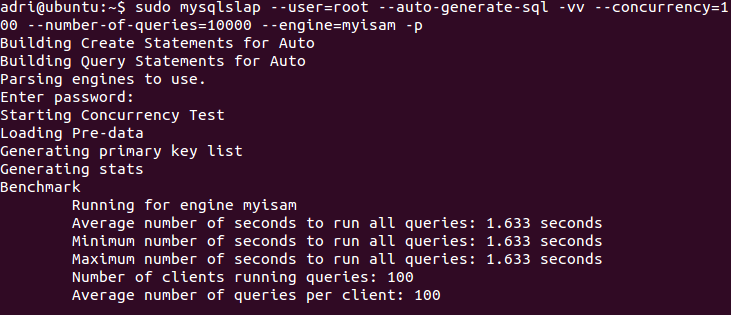
\includegraphics[width=1\linewidth]{sql2.png} 
\caption{Resultado del test usando MyISAM.} 
\label{contexto:figura} 
\end{figure} 

\begin{figure}[H]
\centering 
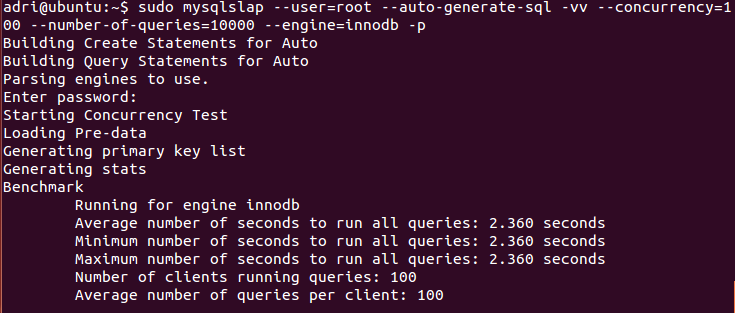
\includegraphics[width=1\linewidth]{sql3.png} 
\caption{Resultado del test usando INNODB.} 
\label{contexto:figura} 
\end{figure} 

Como podemos observar la diferencia es de casi 1s, lo cual es un tiempo a tener en cuenta, por lo que he decidido cambiar el motor de almacenamiento (ya que el que viene por defecto con MySQL es INNODB) por MyISAM, ya que mi servidor no requiere de las funcionalidades adicionales de INNODB y puede funcionar con MyISAM.

Para ello en el fichero que tenemos en \textit{/etc/mysql/my.cnf} añadiremos las siguientes líneas\cite{10}:

\begin{verbatim}
    default-storage-engine=myisam
    skip_innodb
\end{verbatim}
También cabe destacar que el motor MyISAM consume bastante menos memoria RAM que el motor INNODB ya que tiene menos funcionalidades.

\pagebreak

\begin{thebibliography}{99}
\bibitem{1} \url{http://rm-rf.es/sysctl-y-procsys-modificar-parametros-de-kernel/}
\bibitem{2} \url{http://www.programmershare.com/1674057/}
\bibitem{3} \url{http://windows.microsoft.com/es-xl/windows/back-up-registry#1TC=windows-7}
\bibitem{4} \url{http://ss64.com/nt/reg.html}
\bibitem{5} \url{https://support.microsoft.com/es-es/kb/256986}
\bibitem{6} \url{http://docs.moodle.org/23/en/Performance_recommendations}
\bibitem{7} \url{https://technet.microsoft.com/es-es/library/cc730629(v=ws.10).aspx}
\bibitem{8} \url{https://addons.mozilla.org/es/firefox/addon/firebug/}
\bibitem{9} \url{http://linux.die.net/man/1/mysqlslap}
\bibitem{10} \url{http://blog.arsys.es/myisam-o-innodb-elige-tu-motor-de-almacenamiento-mysql/}
\end{thebibliography}
\end{document}
